\documentclass{article}

\usepackage{graphicx, xcolor}
\usepackage{amsmath, amssymb}

\usepackage[margin=1in]{geometry}

\def\hwtitle{Homework 1: Graphing and Introduction}
\def\hwauthor{Caden Gobat}
\def\hwdate{\today}

\usepackage{fancyhdr}
\lhead{\hwauthor}
\chead{\hwtitle}
\rhead{\hwdate}
\lfoot{\hwauthor}
\cfoot{}
\rfoot{\thepage}
\renewcommand{\footrulewidth}{0.4pt}
\pagestyle{fancy}

\author{\hwauthor}
\title{\hwtitle}
\date{\hwdate}

\begin{document}

\maketitle
\thispagestyle{fancy}

\section{Introduction}

In general, if the forces on a body are known, one can derive equations representing its position by solving differential equations using Newton's second law. In the specific case of springs and their oscillatory motion, the force itself depends on the position of the mass. This is apparent from Hooke's Law: $\mathbf{F} = k|r|(-\hat{\mathbf{r}})$. By treating $\mathbf{r}$ as a vector in $(x,y)$ space, and solving some simple second-order linear differential equations, one can obtain the general solution for the $x$ and $y$ positions of the mass throughout time through the vector equation $\displaystyle \langle x(t),\ y(t)\rangle  = \langle A_x\sin(\omega t +\phi_x),\ A_y\sin(\omega t + \phi_y)\rangle$. The two components can be treated essentially independently of one another, and as such we can get a 2D position of the mass for any point $t$ in time, provided we know (or can define) the constants $A_x$, $A_y$, $\omega$, $\phi_x$, and $\phi_y$.

Here I will do exactly this, and plot the results.

\section{Results}

\bigskip
\noindent{\bf Question 1}
\medskip

Submitted for the code assignment. $\checkmark$

\bigskip
\noindent{\bf Question 2}
\medskip

The plots on the following page were generated using the \texttt{C} and \texttt{Mathematica} code submitted for the code assignment. Each row represents a different phase difference ($\Delta\phi$) requested in the assignment, while the two columns represent $(A_x,A_y)=(1,1)$ and $(A_x,A_y)=(2,1)$, respectively. Note the scaling of the axes between plots, as the shapes themselves can appear deceptively similar.

\bigskip
\noindent{\bf Question 3}
\medskip

In general, it seems like these equations tend to produce ellipses of various kinds. $A_x$ and $A_y$ affect the scaling in each direction (indirectly, the semi-major and semi-minor axes), and the phase difference $\Delta\phi$ affects the eccentricity and angle of the ellipse. The frequency $\omega$ only affects the ``speed'' at which the mass travels, not the actual shape of its path. As such, it was held constant due to the fact that it has little discernible impact on the appearance of the plots (besides the spacing between each point in time, which is not conveyed in this ``strobe light''-style plot). Perhaps an animation would help to illustrate this concept further.

It seems that $\Delta\phi = n\pi$, where $n=0,1,2,3,...$ produces a line (essentially an ellipse with eccentricity$=1$), while $\Delta\phi=\frac{n\pi}{2}$, whereas $n=1,3,5,...$ creates circles (assuming $A_x=A_y$, otherwise just an ellipse with its axes aligned with the $x$- and $y$-axes). Other phase differences produce ellipses of various eccentricities (and, as long as $A_x=A_y$, the semi-major axis will be aligned with either $y=x$ or $y=-x$).

\begin{tabular}{ll}
    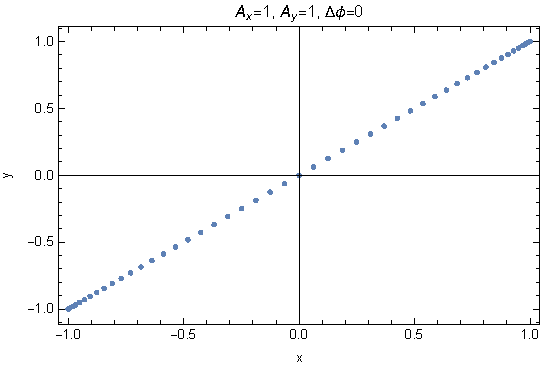
\includegraphics[width=3in]{homework1/plot_1,1,0.pdf} & 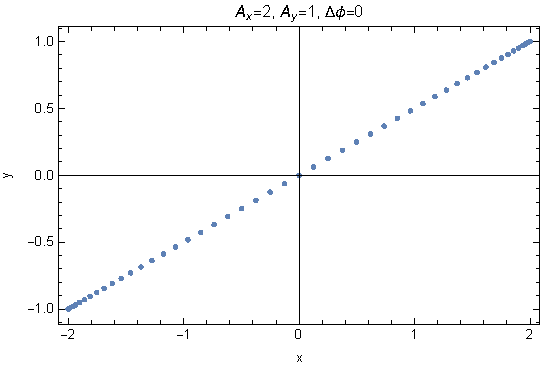
\includegraphics[width=3in]{homework1/plot_2,1,0.pdf} \\
    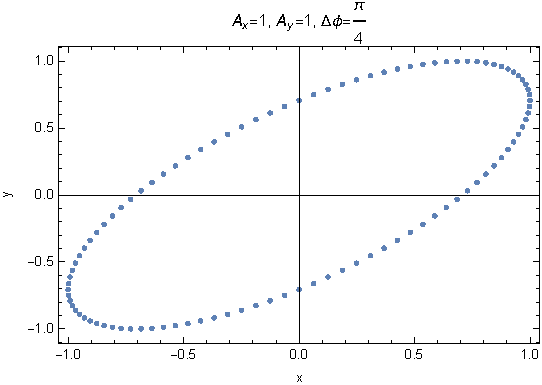
\includegraphics[width=3in]{homework1/plot_1,1,pi4.pdf} & 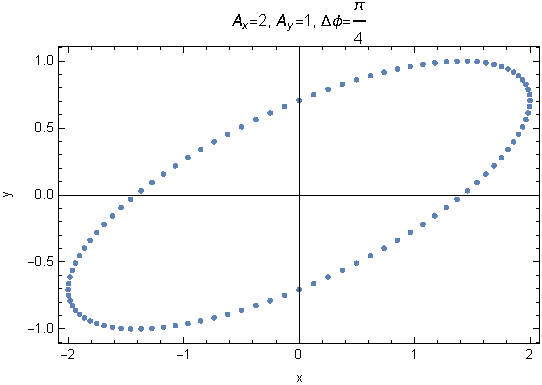
\includegraphics[width=3in]{homework1/plot_2,1,pi4.pdf} \\
    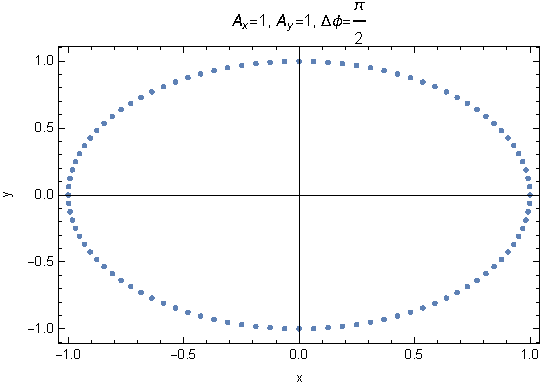
\includegraphics[width=3in]{homework1/plot_1,1,pi2.pdf} & 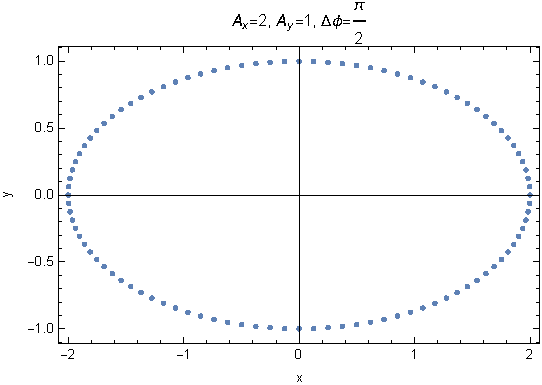
\includegraphics[width=3in]{homework1/plot_2,1,pi2.pdf} \\
    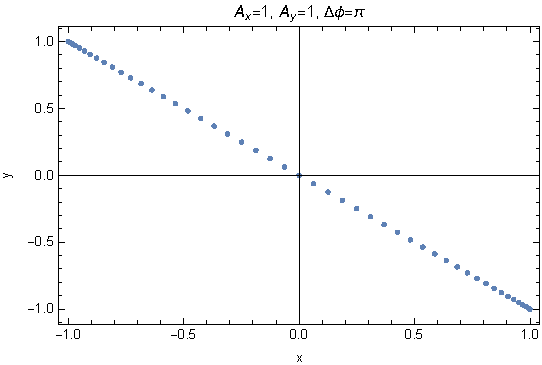
\includegraphics[width=3in]{homework1/plot_1,1,pi.pdf} & 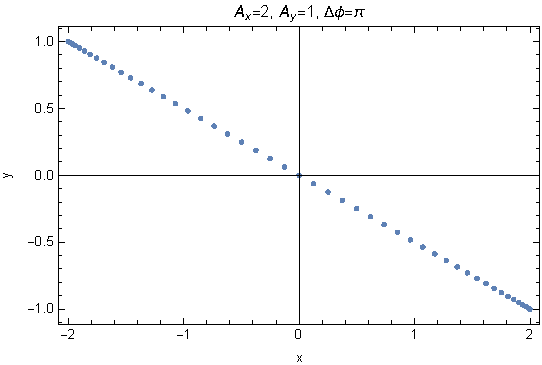
\includegraphics[width=3in]{homework1/plot_2,1,pi.pdf}
\end{tabular}

\newpage

\noindent{\bf Bonus problem}
\medskip

The following plots of Lissajous figures were created using a similar setup, but with $\omega_x \neq \omega_y$. The parameters that varied in the previous problems were held constant here, while the ratio $\frac{\omega_x}{\omega_y}$ was manipulated to create the shapes seen here. The time domain was set to run from $0 \leq t \leq \frac{50}{\omega_\text{min}}$ in each case.

\begin{center}
    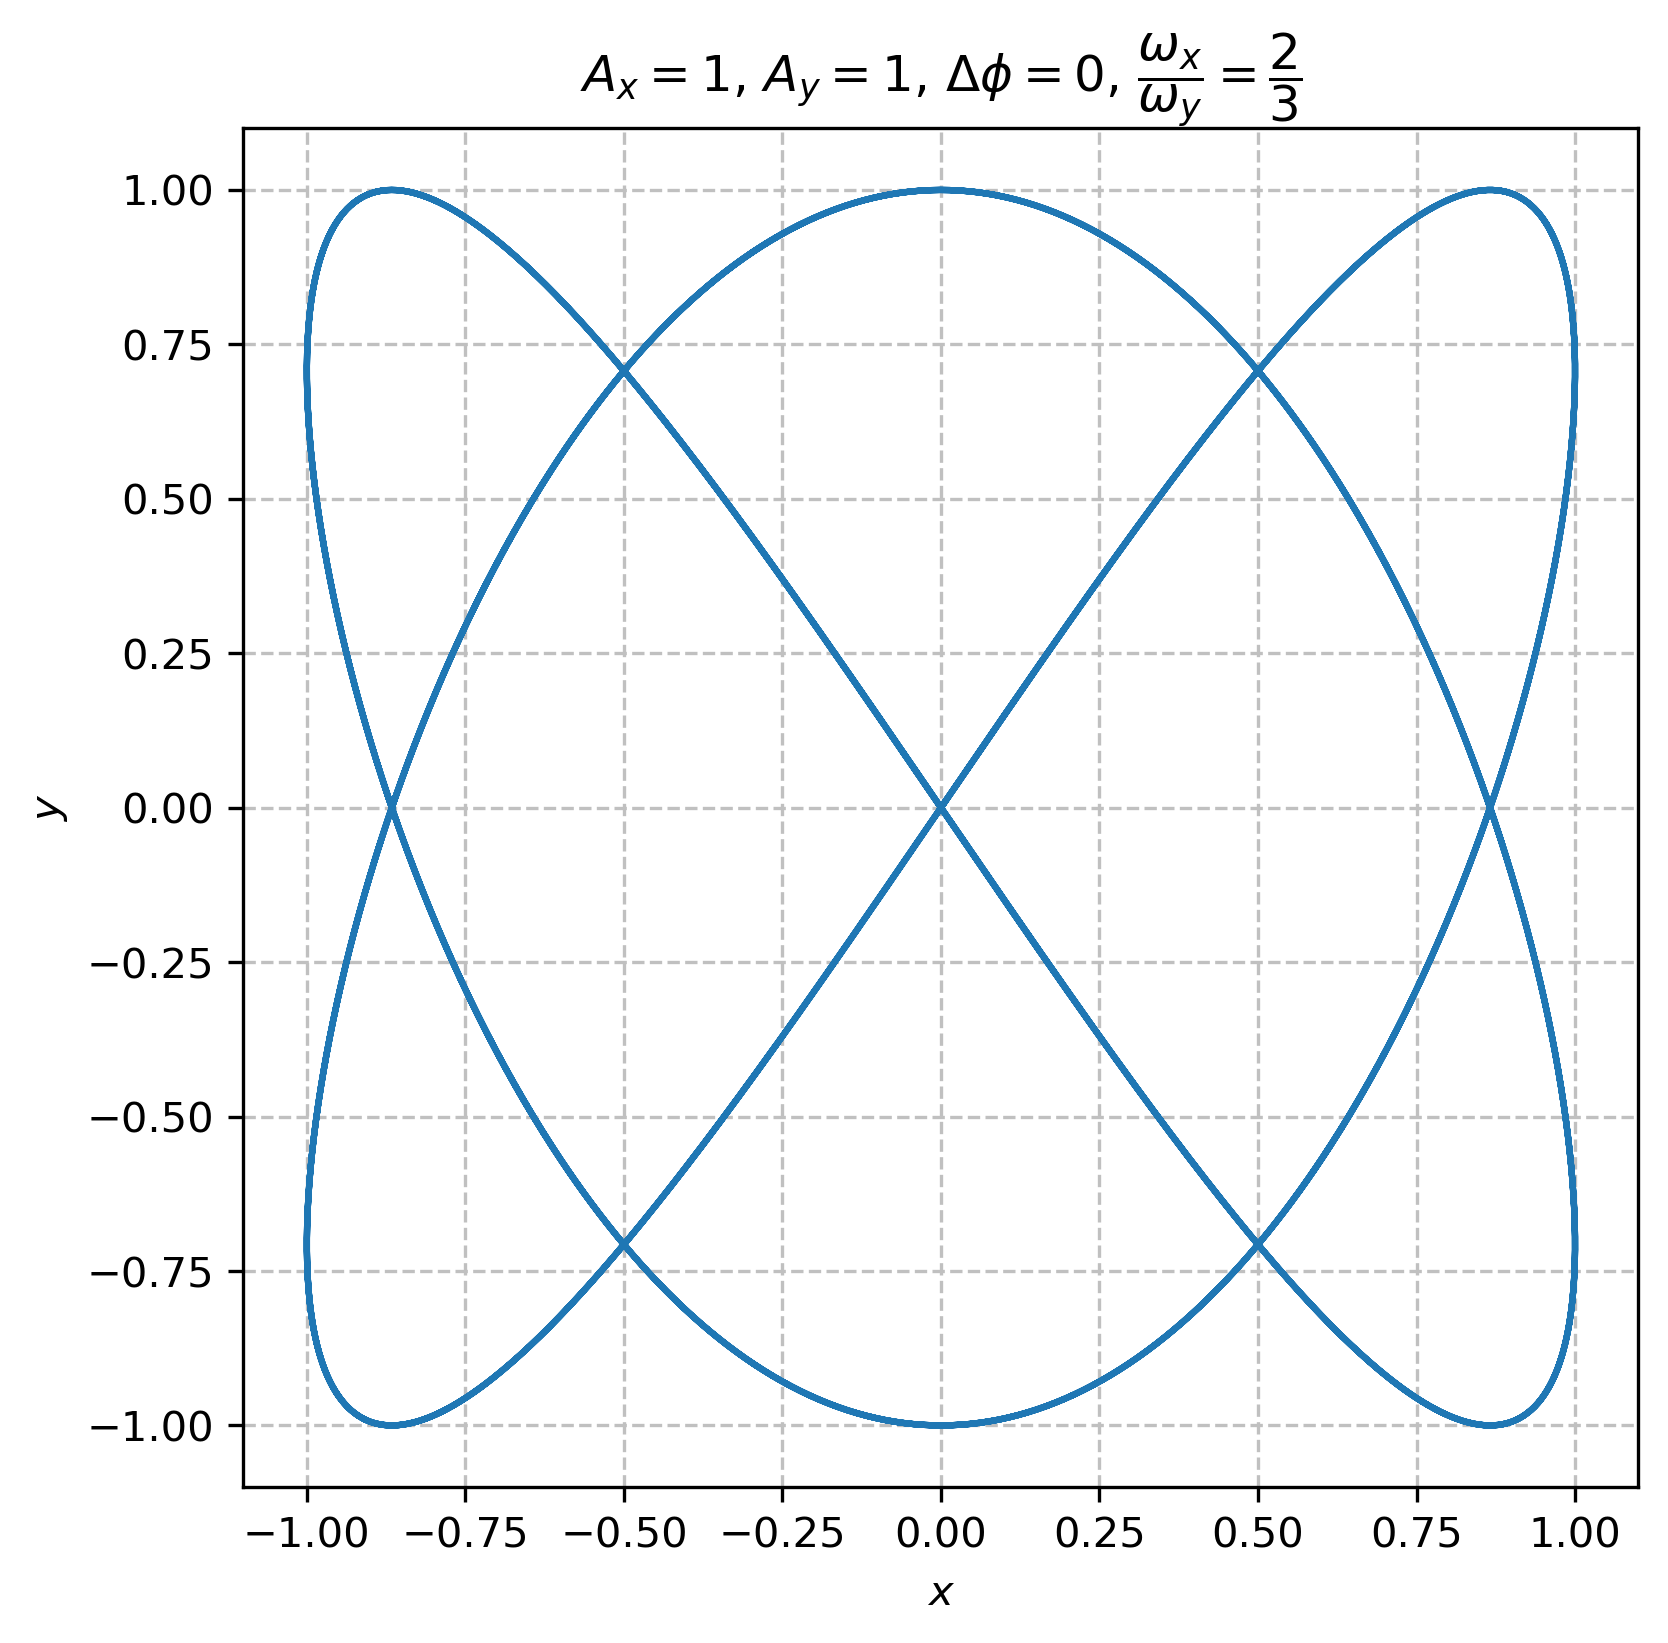
\includegraphics[width=3.2in]{homework1/lissajous_2-3.png}
    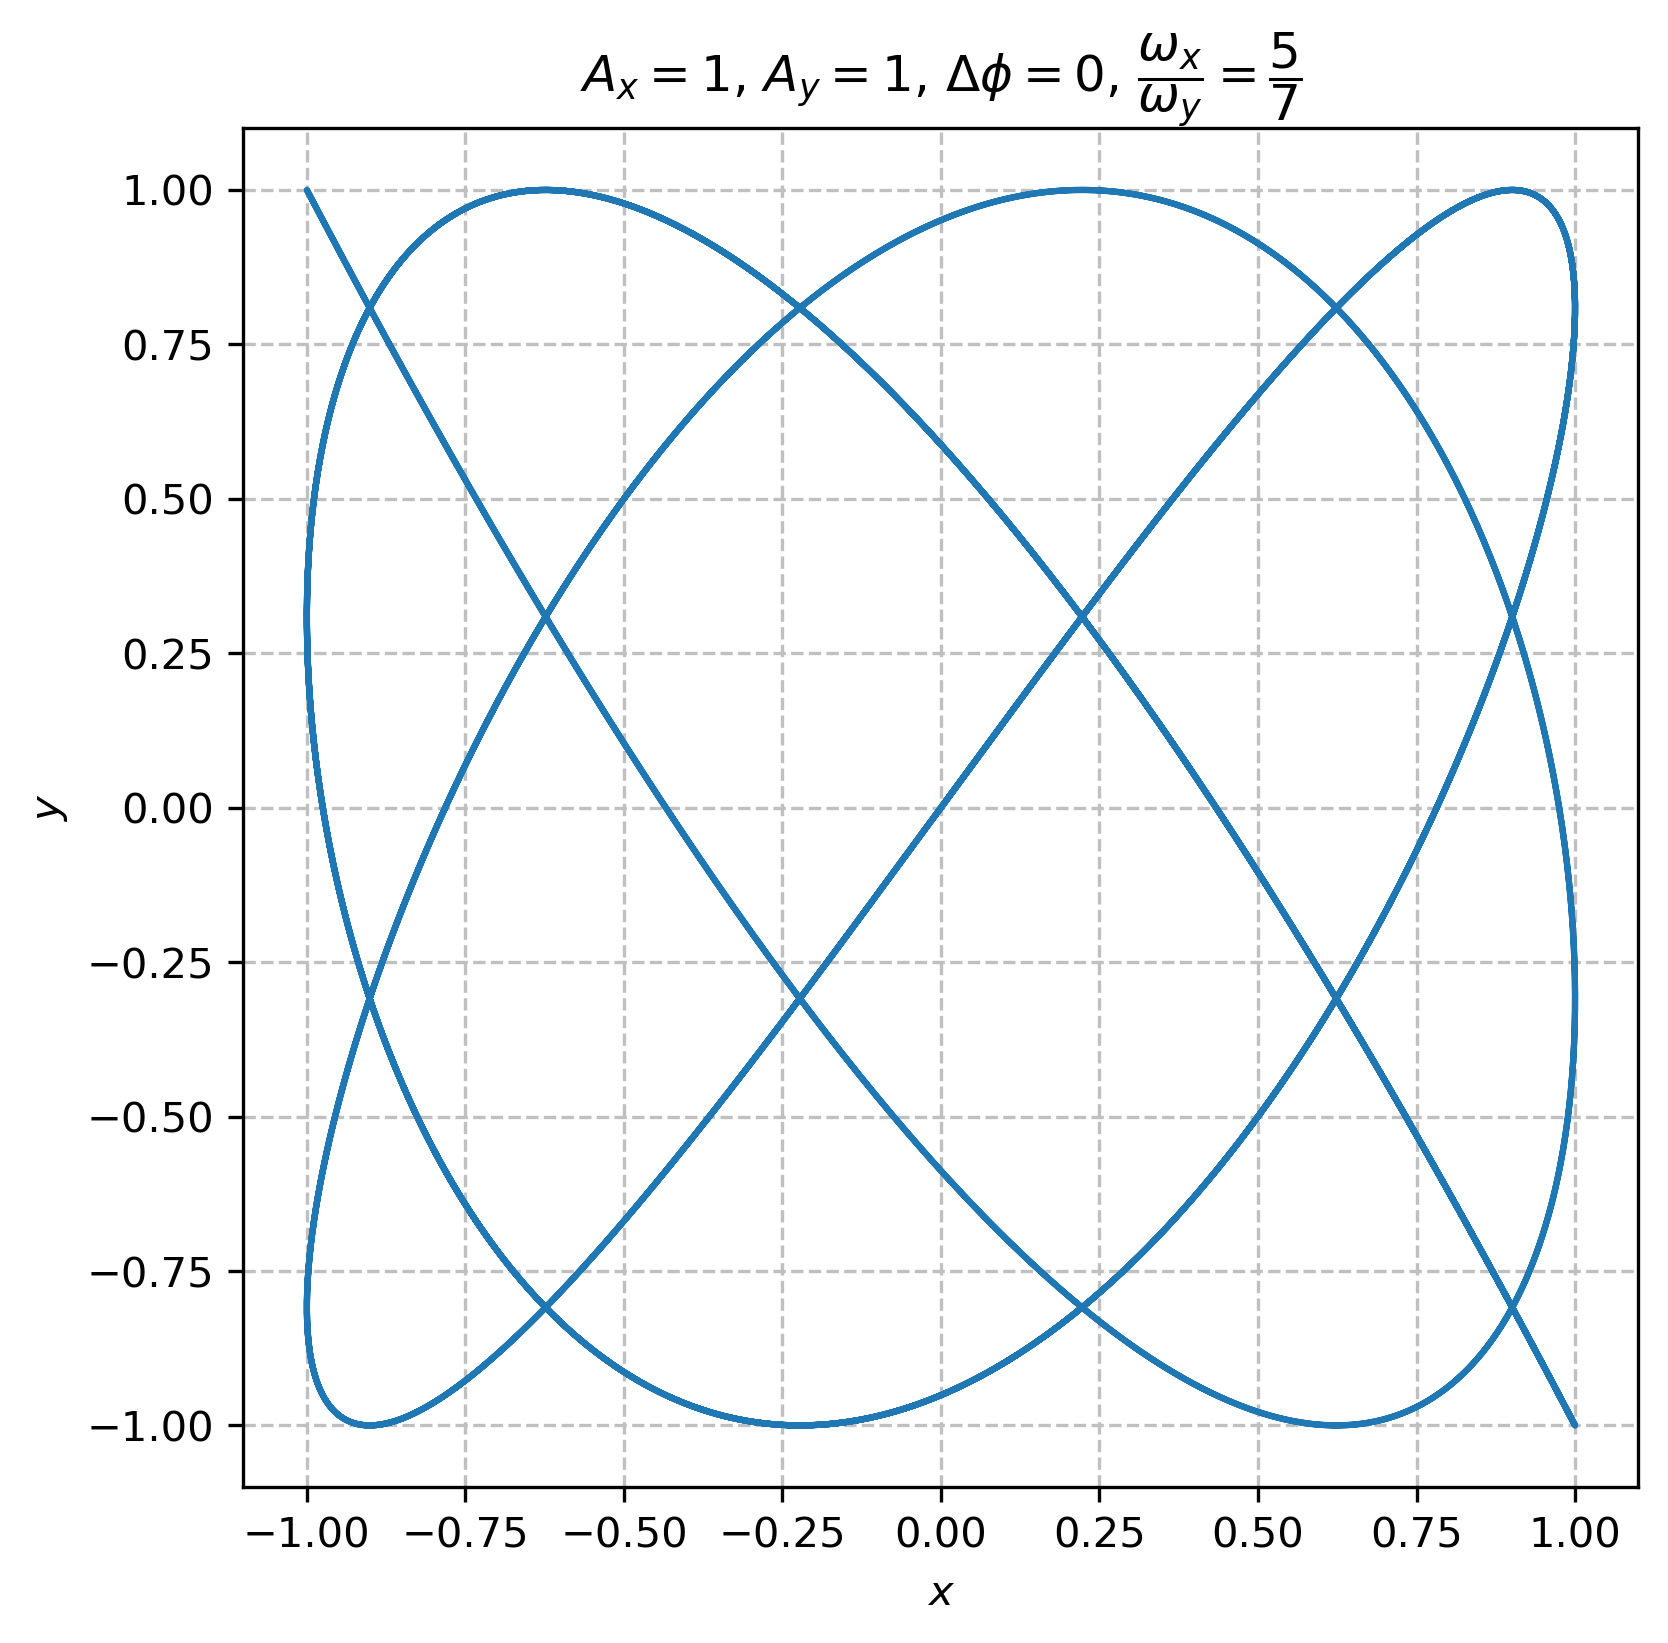
\includegraphics[width=3.2in]{homework1/lissajous_5-7.png}
    
    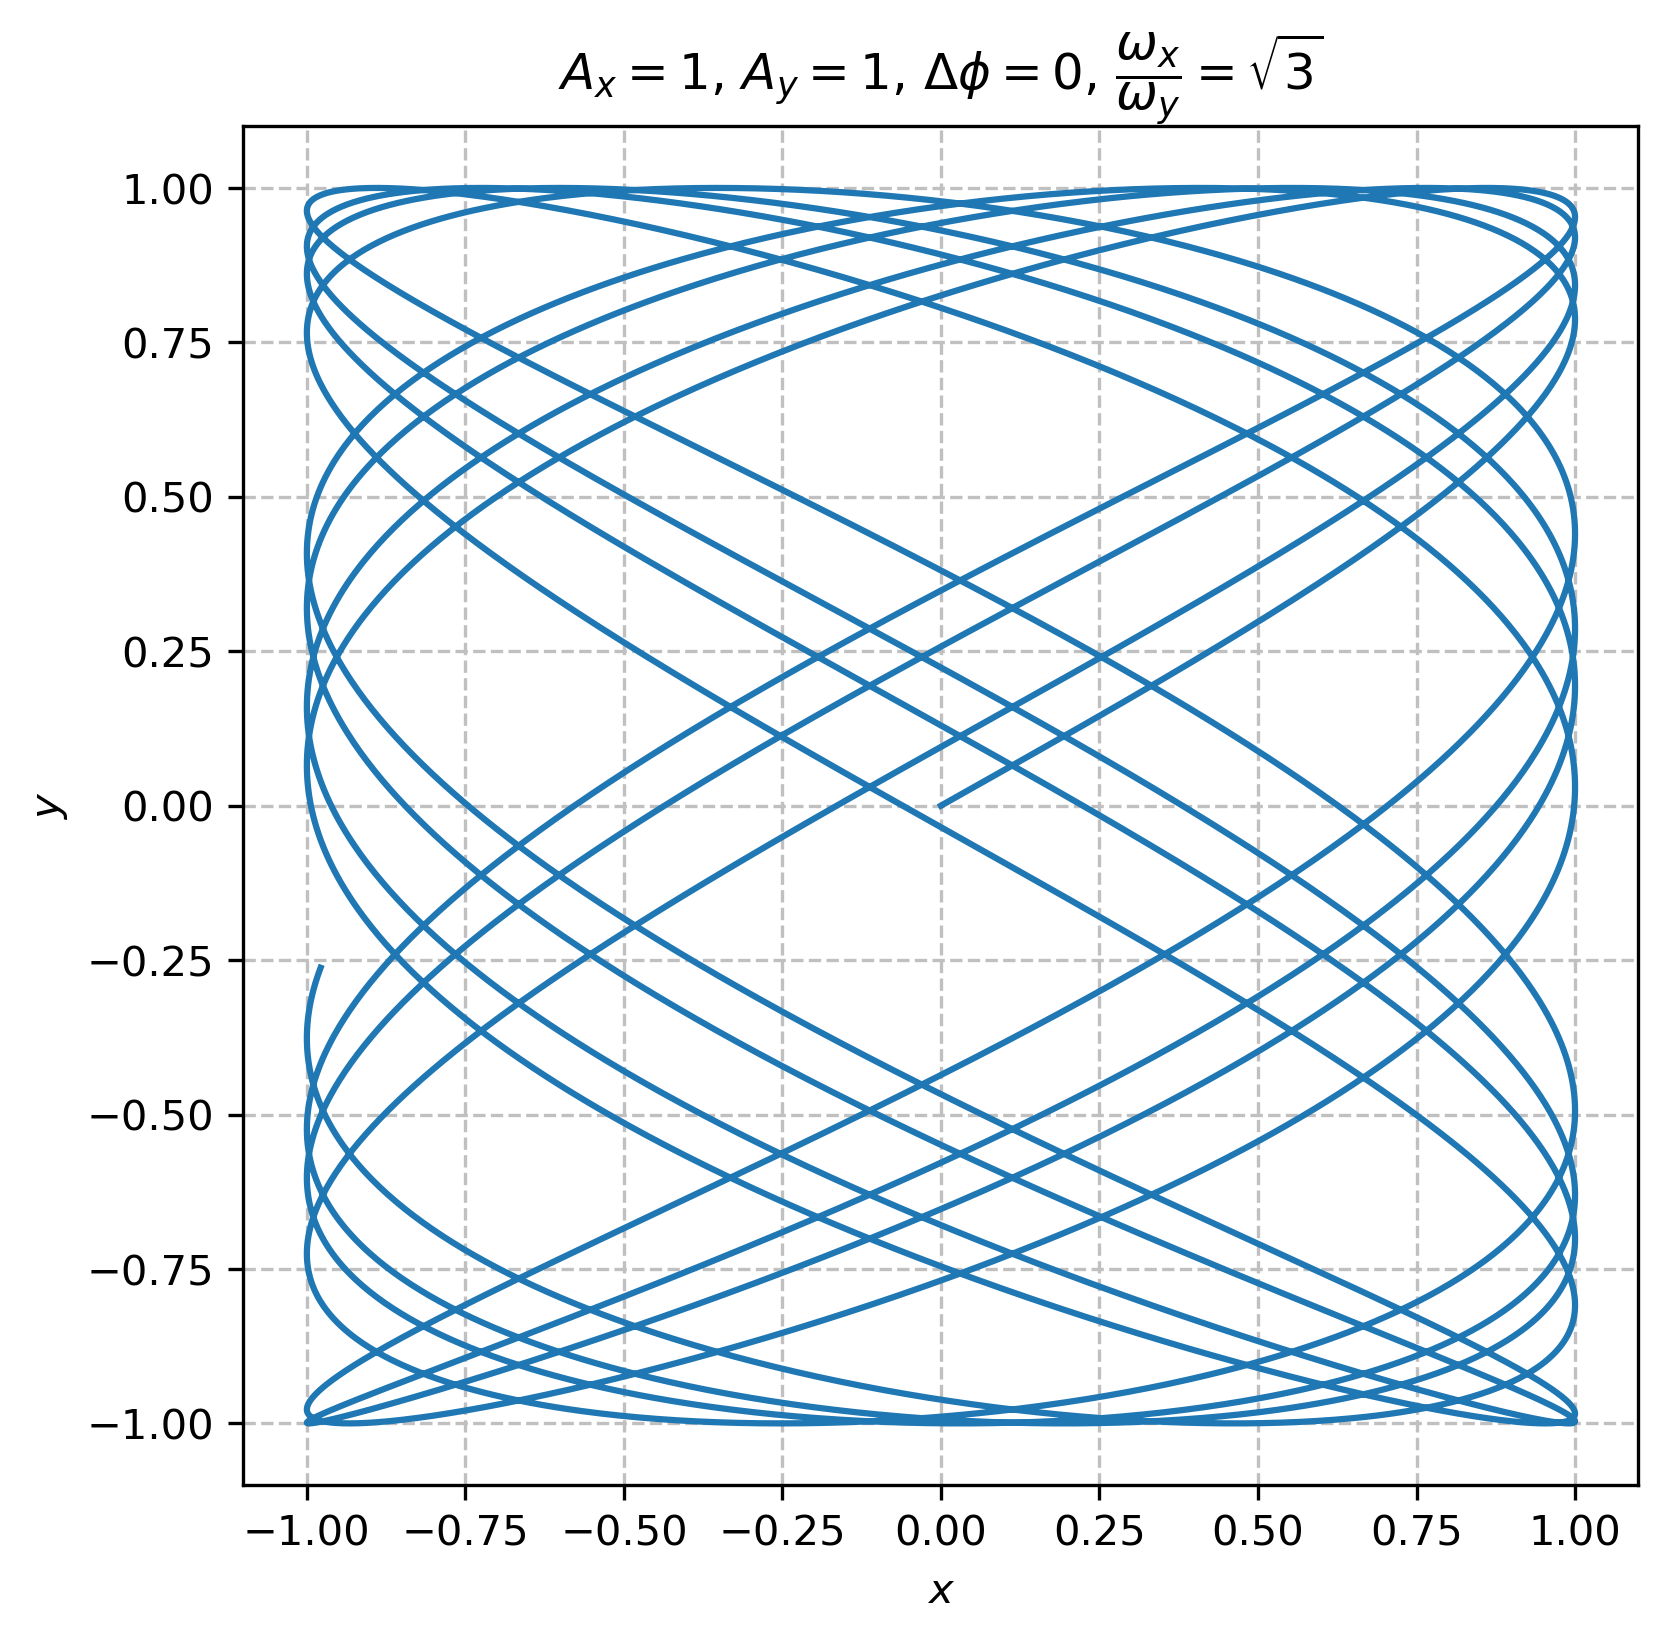
\includegraphics[width=3.2in]{homework1/lissajous_sqrt3.png}
\end{center}

Rational values of $\frac{\omega_x}{\omega_y}$ (such as $\frac{2}{3}$ and $\frac{5}{7}$) produce figures where the same shape is traced out, period after period. It seems that if the numerator is even, it creates a ``closed loop'' where there are no apparent endpoints (seen in the first figure above), while odd numerators create more of an open-ended line, as in the second figure.

Irrational values of the frequency ratio, such as $\frac{\omega_x}{\omega_y}=\sqrt{3}$, mean that the traced path is not the same each period. This results in a sort of drift over time, as the last figure above shows.

\section{Conclusions}

In all, this assignment constituted a good introduction to the principles of computation in \texttt{C} and subsequent visualization in \texttt{Mathematica}. I ran into some issues initially because it seems that math constants like \texttt{M\_PI} are not available in the \texttt{c99} implementation, so one must either define it manually (something along the lines of \texttt{\#define PI 4.*atan(1)}) or use a different standard when compiling. Depending on the operating system I was working on, I found that I sometimes had to pass the \texttt{-lm} flag to get the math library to link properly as well.

Importing the generated data into \texttt{Mathematica} also presented some trouble at first because I was formatting it as comma-separated, which apparently the \texttt{ReadList[]} function is unable to parse. Switching to tab-separated values in the \texttt{C} code output resolved the issue.

Besides these minor technical issues, the project went well and I was able to complete it successfully and with an improved understanding of the softwares involved.

\end{document}
